\documentclass[conference]{IEEEtran}
\IEEEoverridecommandlockouts
\usepackage[utf8]{inputenc}
\usepackage[T1]{fontenc}
\usepackage{cite}
\usepackage{amsmath,amssymb,amsfonts}
\usepackage{algorithmic}
\usepackage{graphicx}
\usepackage{textcomp}
\usepackage{booktabs}
\usepackage{tabularx}
\usepackage{adjustbox}
\usepackage{hyperref}
\hypersetup{hidelinks}
\usepackage[dvipsnames]{xcolor}
\usepackage{array}
\usepackage{multirow}
\usepackage{pifont}
\usepackage{url}
\newcommand{\cmark}{\ding{51}}%
\newcommand{\xmark}{\ding{55}}%
\def\BibTeX{{\rm B\kern-.05em{\sc i\kern-.025em b}\kern-.08em
    T\kern-.1667em\lower.7ex\hbox{E}\kern-.125emX}}
\begin{document}

\title{Adaptive Data Movement Strategy Selection for AES Accelerator Workloads on STM32-Class MCUs}

\author{\IEEEauthorblockN{Süleyman Ege Karakaya}
\IEEEauthorblockA{Computer Engineering Department Hacettepe University, Ankara, Turkiye\\
Graduate School of Science and Engineering Hacettepe University, Ankara, Turkiye\\
segekarakaya26@hacettepe.edu.tr}}

\maketitle

\begin{abstract}
Cryptographic acceleration is common in secure embedded systems, but the end-to-end performance of such systems is often dominated by data movement rather than raw cryptographic computation. This final report studies how an STM32-class microcontroller can choose among programmed I/O, DMA single-shot, DMA burst, and simulated double-buffer transfer strategies when invoking AES accelerator workloads under different payload sizes and resource conditions. The original extended proposal targeted an STM32H7-class MCU and included both AES and ECDSA workloads. In the final implementation, the concrete hardware prototype was completed on an STM32F439ZI board using the on-chip AES CRYP peripheral; ECDSA and true hardware double buffering were not completed and are therefore reported as limitations. The project formulates transfer-mode selection as a weighted optimization problem over latency, CPU occupancy, and bus pressure, and implements a lightweight selector that evaluates feasible modes and returns the minimum-cost choice. Simulation results show that the adaptive selector matched the oracle decision for CPU-dominant, latency-dominant, and equal-weight configurations. Real AES measurements on 50 REAL\_3WAY jobs show that static DMA single-shot had the lowest average latency and highest average throughput on the measured workload, while the adaptive selector provided mixed-mode behavior and avoided the very poor performance of static PIO. The results confirm that transfer-mode choice is workload-dependent and that an adaptive policy is useful, but they also show that the selector must be calibrated with real measurements when the hardware implementation differs from the simulation model.
\end{abstract}

\begin{IEEEkeywords}
embedded systems, cryptographic accelerator, DMA, AES, data movement optimization, STM32
\end{IEEEkeywords}

\section{Introduction}
Modern embedded platforms increasingly rely on hardware-assisted cryptography for secure boot, firmware authentication, secure storage, and protected communication. In these systems, standardized primitives such as AES and ECDSA are attractive because they are widely deployed and supported by both software and hardware implementations \cite{fips197,fips1865}. However, accelerator-centric performance discussions often focus on the compute core alone, even though end-to-end latency also depends on how input data, descriptors, control words, and results move across the processor, memory system, DMA engine, and accelerator interface.

This issue is especially important in MCU-class systems. Compared with application processors, STM32-class devices operate under tighter memory, buffering, and bus contention constraints. A fixed data-movement strategy is therefore rarely optimal across all cryptographic requests. Very small messages may not amortize DMA setup overhead, while larger AES buffers benefit from DMA-based movement or overlapped execution. The practical design question is not only whether hardware AES is fast, but also which transfer path should be used for a given job.

The central question of this work is the following: \emph{given a cryptographic job, payload size, and resource state, which transfer strategy minimizes a system-level cost when AES acceleration is invoked from an STM32-class embedded system?} This final report continues the extended proposal by turning the optimization formulation into a simulation and measurement workflow. The final project produced: (1) a weighted-cost selector, (2) simulation studies under different metric priorities, and (3) real AES measurements comparing adaptive selection against static PIO, static DMA single-shot, and static DMA burst baselines.

The final scope is narrower than the initial proposal. The original proposal included both AES and ECDSA and targeted an STM32H7-class architecture. The completed hardware measurements focus on AES on an STM32F439ZI board. ECDSA, direct power measurement, queue-level scheduling, and true hardware double buffering remain future work.

\section{Related Work}
This review organizes the literature around three themes relevant to the project: accelerator-centric cryptographic design, DMA/interconnect-aware data movement, and adaptive hardware/software execution. The purpose of the review is to clarify what has already been optimized and what gap remains open for MCU-level cryptographic offload.

\subsection{Embedded Cryptographic Acceleration}
A first body of work improves cryptographic performance by redesigning the accelerator itself. Zhang \emph{et al.} address real-time protection of streaming data by integrating a parallel AES-GCM engine into an embedded security SoC, showing that internal datapath parallelism can substantially increase throughput \cite{zhang2021}. For public-key workloads, Agrawal \emph{et al.} accelerate FPGA-based ECDSA verification through custom arithmetic pipelines and optimized elliptic-curve point operations \cite{agrawal2022}. These studies show that accelerator microarchitecture strongly affects latency and throughput. Their limitation with respect to this project is that the host-to-accelerator transfer path is usually assumed to be fixed or already efficient.

\subsection{DMA and Interconnect-Aware Embedded Design}
A second theme studies the cost of moving data inside embedded systems. Vendor documentation and architecture guides show that DMA can reduce CPU intervention and improve burst efficiency when it is aligned with the underlying memory and interconnect structure \cite{silabs_dma,arm_axi}. Saidi \emph{et al.} highlight that DMA scheduling, locality, and transfer orchestration are major performance factors in embedded multi-core systems \cite{Saidi2012}. Mera \emph{et al.} add a security perspective by showing that DMA introduces multi-master access behavior that affects isolation and protection mechanisms \cite{Mera2022}. Together, these works motivate treating data movement as a first-class design variable rather than a transparent implementation detail.

\subsection{Adaptive and Reconfigurable Embedded Frameworks}
A third line of work explores adaptive hardware/software execution. The ARTICo$^3$ framework shows how FPGA-based embedded systems can dynamically manage acceleration resources in cyber-physical settings \cite{Rodrguez2018}. SmartDMA extends this perspective to programmable data movement and argues that flexible memory-access engines are beneficial when workload behavior changes across edge scenarios \cite{Zulberti2024}. Hardware/software co-design studies for modern cryptography also show that end-to-end benefit depends on how responsibilities are partitioned across software and hardware \cite{Montanaro2022}. These works support the idea that static execution policies are often suboptimal, but they usually operate at a coarser granularity than the per-job transfer-mode decision studied here.

\subsection{Positioning of This Work}
The project combines the above insights at a practical MCU level. Rather than designing a new cipher core, it evaluates how an STM32-class host should choose among feasible transfer mechanisms when dispatching AES jobs to a hardware accelerator. Table~\ref{tab:related_work} summarizes the positioning. The final implementation does not fully realize the original AES/ECDSA scope; it validates the methodology using AES hardware measurements and simulation-based sensitivity analysis.

\begin{table}[ht!]
\centering
\caption{Representative related studies and positioning of this work.}
\label{tab:related_work}
\scriptsize
\setlength{\tabcolsep}{3pt}
\begin{adjustbox}{width=\columnwidth}
\begin{tabular}{p{2.15cm} p{0.8cm} p{1.35cm} p{2.0cm} p{1.95cm} p{2.10cm}}
\toprule
\textbf{Work} & \textbf{Year} & \textbf{Platform} & \textbf{Method / Focus} & \textbf{Metric / Result} & \textbf{Limitation w.r.t. This Work} \\
\midrule
Zhang \emph{et al.}~\cite{zhang2021} & 2021 & Embedded SoC & Parallel AES-GCM accelerator datapath & Higher streaming throughput & Transfer-mode selection is not studied \\
Agrawal \emph{et al.}~\cite{agrawal2022} & 2022 & FPGA & Pipelined ECDSA verification & Lower verification latency & Limited MCU-side transfer-path analysis \\
Saidi \emph{et al.}~\cite{Saidi2012} & 2012 & Embedded multi-core & DMA scheduling and locality & Better transfer efficiency & Not cryptography-specific \\
Mera \emph{et al.}~\cite{Mera2022} & 2022 & Embedded systems & DMA-aware isolation & Highlights DMA security concerns & Security-centric, not mode optimization \\
Rodriguez \emph{et al.}~\cite{Rodrguez2018} & 2018 & FPGA CPS/edge & Adaptive reconfigurable acceleration & Dynamic resource management & Coarser-grained than per-job selection \\
Zulberti \emph{et al.}~\cite{Zulberti2024} & 2024 & Edge architectures & Programmable memory-access controller & Adaptable data movement & Not focused on MCU AES jobs \\
Montanaro \emph{et al.}~\cite{Montanaro2022} & 2022 & HW/SW crypto & Accelerator/software partitioning & Boundary management matters & No explicit transfer-mode optimizer \\
\textbf{This work} & 2026 & STM32-class MCU & Per-job AES transfer-mode selection & Latency, throughput, regret, deadline miss & ECDSA and true double buffering not completed \\
\bottomrule
\end{tabular}
\end{adjustbox}
\end{table}

\section{Problem Definition}
\subsection{System / Application Description}
The target application domain is a secure embedded node that invokes cryptographic operations for bulk protection and identity-related tasks. The original reference architecture was an STM32H745-class MCU with on-chip SRAM, DMA support, and a memory-mapped cryptographic accelerator interface. In the final project, the implemented measurement platform was an STM32F439ZI board using the internal CRYP AES hardware block. The system-level problem remains the same: each job arrives with a payload size and a resource state, and the runtime must choose a data-movement mode.

The final measured workload focuses on AES jobs. ECDSA jobs were retained in the conceptual problem statement but were not measured on hardware. This distinction is important because ECDSA-style workloads would likely have different transfer characteristics: they are smaller, more descriptor-heavy, and less throughput-oriented than bulk AES.

\subsection{Objectives}
The primary objective is to choose a transfer mode that minimizes end-to-end cost for a cryptographic job. Cost is defined by latency, CPU occupancy, and bus pressure. The project has four concrete objectives:
\begin{enumerate}
    \item characterize the performance region in which each transfer strategy is preferable,
    \item formulate transfer-mode selection as a constrained optimization problem,
    \item implement a lightweight selector suitable for an MCU runtime, and
    \item compare adaptive selection against static transfer-mode baselines.
\end{enumerate}

\subsection{Constraints}
The optimization is constrained by embedded-system realities: limited SRAM, DMA setup overhead, DMA channel availability, bus bandwidth, contention, response-time requirements, and implementation simplicity. DMA-based modes are not always beneficial because small payloads may not amortize setup and synchronization costs. Double buffering also requires two buffers plus metadata and was not implemented in the final hardware experiment.

\subsection{Decision Variables and Optimization Model}
Let $J$ denote the set of cryptographic jobs and $M$ denote the candidate transfer modes. In the full model,
\begin{equation}
M = \{\text{PIO}, \text{DMA-SS}, \text{DMA-Burst}, \text{DoubleBuffer}\}.
\end{equation}
A job $j \in J$ is described by algorithm label $a_j$, payload size $s_j$, contention class $c_j$, and deadline or response-time requirement $d_j$. A binary decision variable $x_{j,m}$ indicates whether job $j$ uses mode $m$:
\begin{equation}
x_{j,m} = \begin{cases}
1, & \text{if job } j \text{ is executed using mode } m,\\
0, & \text{otherwise.}
\end{cases}
\end{equation}

Feasibility is handled before weighted-cost minimization. The decision variable $x_{j,m}$ is allowed to become one only when the corresponding mode satisfies the platform and job-level feasibility inputs summarized in Table~\ref{tab:feasibility_inputs}. These values are not optimized by the selector; they are measured, configured, or estimated from the current platform state.

\begin{table}[ht!]
\centering
\caption{Feasibility inputs used by the transfer-mode selector.}
\label{tab:feasibility_inputs}
\begin{tabularx}{\linewidth}{@{}lX@{}}
\toprule
Symbol & Meaning \\
\midrule
$A_{j,m}$ & Alignment and block-size validity. For AES, payload sizes must respect the 16-byte block granularity required by the hardware CRYP path. \\
$D_{j,m}$ & DMA-resource availability, including whether a DMA-based mode can be configured safely for the requested transfer. PIO does not require this resource. \\
$R_{j,m}$ & SRAM and buffer availability. Double buffering requires two buffers and additional control metadata, while single-buffer modes have lower memory demand. \\
$Q_{j,m}$ & Contention and queue-state compatibility, representing whether the current background load allows the mode to be used without violating the assumed resource model. \\
$T_{j,m}$ & Timing feasibility, defined as one when the estimated latency does not exceed the job deadline, i.e., $L(j,m) \leq d_j$, when the deadline is enforced as a hard constraint. \\
\bottomrule
\end{tabularx}
\end{table}

The combined feasibility indicator is defined as
\begin{equation}
f_{j,m} = A_{j,m} D_{j,m} R_{j,m} Q_{j,m} T_{j,m}.
\label{eq:feasibility_indicator}
\end{equation}
If deadline is evaluated only as a reporting metric rather than a hard constraint, $T_{j,m}$ is set to one during selection and deadline miss is reported separately as $\mathbb{1}[L(j,m)>d_j]$. This distinction is important because the simulations used deadline miss rate as an evaluation metric, while a safety-critical deployment could instead use $T_{j,m}$ to eliminate deadline-violating modes before cost comparison.

The objective is to minimize total weighted cost:
\begin{equation}
\min \sum_{j \in J} \sum_{m \in M} x_{j,m} \cdot C(j,m)
\label{eq:objective}
\end{equation}
subject to one selected mode per job,
\begin{equation}
\sum_{m \in M} x_{j,m} = 1 \qquad \forall j \in J,
\label{eq:one_mode}
\end{equation}
and feasibility constraints,
\begin{equation}
x_{j,m} \leq f_{j,m} \qquad \forall j \in J, \forall m \in M.
\label{eq:feasible}
\end{equation}
The per-job cost is modeled as
\begin{equation}
C(j,m) = w_L \hat{L}(j,m) + w_U \hat{U}(j,m) + w_B \hat{B}(j,m),
\label{eq:cost}
\end{equation}
where $\hat{L}(j,m)$ is normalized latency, $\hat{U}(j,m)$ is normalized CPU occupancy, and $\hat{B}(j,m)$ is normalized bus pressure. The online selector returns $\arg\min_{m \in F_j} C(j,m)$ over the feasible set $F_j = \{m \in M \mid f_{j,m}=1\}$.

\section{System Architecture and Design}
\subsection{Hardware/Software Architecture}
The architecture contains application tasks, a runtime selector, the MCU control layer, SRAM buffers, a DMA engine, and a cryptographic accelerator service. Background memory traffic is modeled as a contention source. The selector receives job descriptors and chooses a transfer mode before the dispatcher interacts with the DMA engine or performs direct register accesses. Figure~\ref{fig:architecture} shows the architecture used to frame the project.

\begin{figure}[ht!]
    \centering
    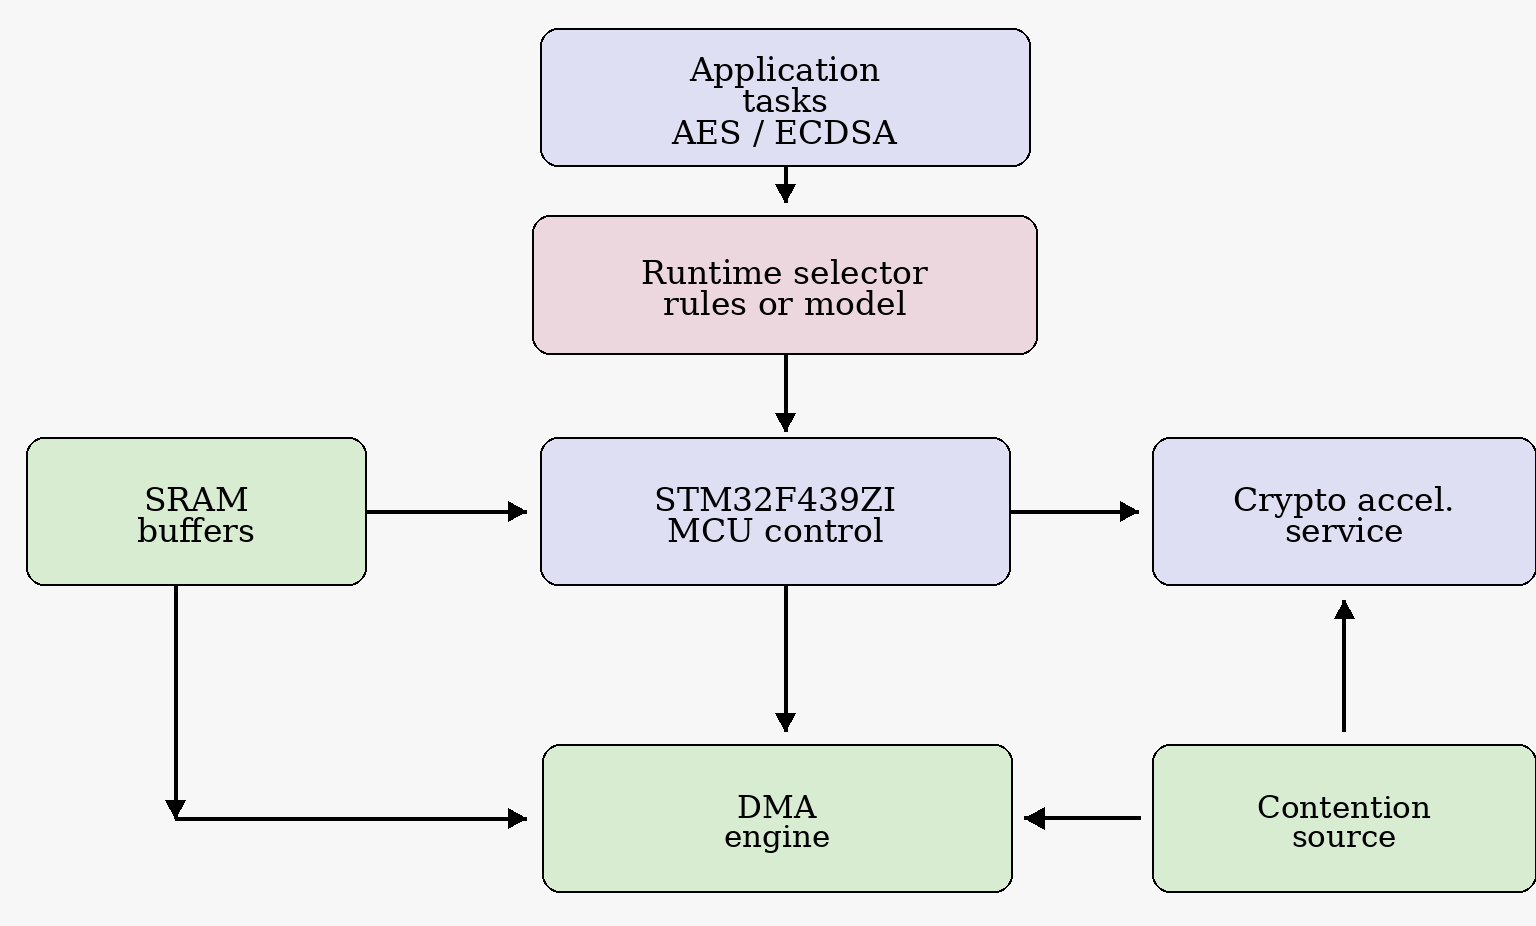
\includegraphics[width=\linewidth]{figures/architecture.png}
    \caption{System architecture for adaptive transfer-mode selection.}
    \label{fig:architecture}
\end{figure}

\subsection{Dataflow and System Model}
The system follows a request-dispatch-complete pattern. A job descriptor is produced by the application layer, the selector estimates the best mode, the MCU prepares descriptors or control words, and the chosen path moves data to the accelerator. The dataflow is event-driven at the software-control level and dataflow-oriented at the buffer-movement level. Figure~\ref{fig:dataflow} summarizes this pipeline.

\begin{figure}[ht!]
    \centering
    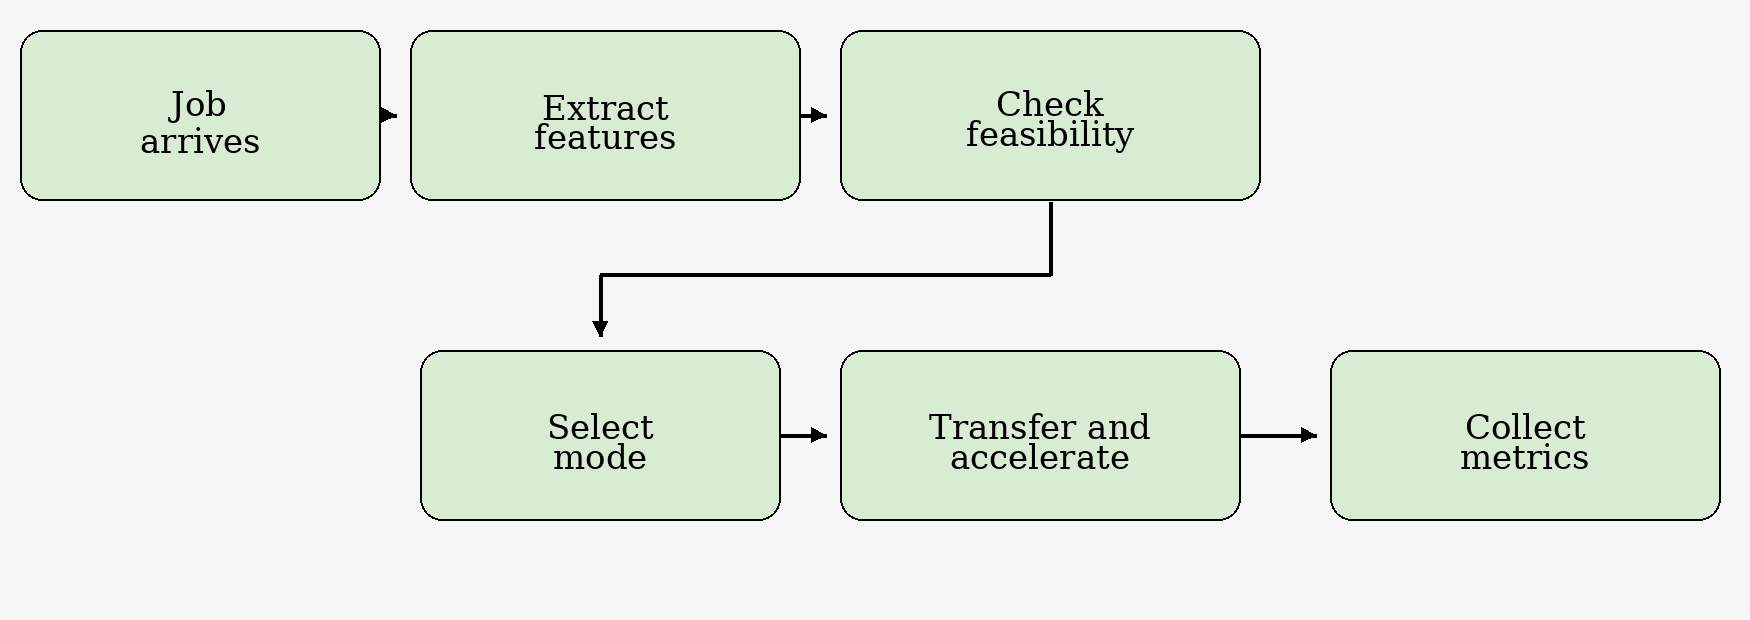
\includegraphics[width=\linewidth]{figures/dataflow.png}
    \caption{Runtime dataflow of the adaptive selection pipeline.}
    \label{fig:dataflow}
\end{figure}

\subsection{Timing and Execution Model}
Cryptographic requests arrive as jobs. For each job, the runtime extracts features, checks feasibility, estimates the cost of available modes, and dispatches the chosen mode. The timing model separates setup cost, data movement, accelerator execution, and synchronization:
\begin{equation}
L(j,m) = T^{\text{setup}}_m + T^{\text{move}}(a_j,s_j,c_j,m) + T^{\text{accel}}(a_j,s_j) + T^{\text{sync}}_m.
\label{eq:latencymodel}
\end{equation}
In the hardware experiment, total latency was measured directly using cycle counts converted to microseconds.

\subsection{Resource Model}
The relevant resources are SRAM, DMA availability, MCU cycles, and bus bandwidth. SRAM constrains buffering depth, DMA availability constrains transfer overlap, MCU cycles capture the cost of PIO-heavy approaches, and bus bandwidth determines whether large transfers are efficient or intrusive. In the final implementation, power was not directly measured; CPU occupancy and transfer count were treated as energy-related proxies in simulation.

\section{Methodology}
\subsection{Optimization Pipeline}
The methodology contains five stages:
\begin{enumerate}
    \item \textbf{Workload generation:} define AES jobs with varying payload sizes and contention labels.
    \item \textbf{Profiling:} measure or estimate latency, CPU occupancy, and bus pressure for each transfer mode.
    \item \textbf{Offline optimization:} label each profiled case with the best mode according to the weighted objective in~\eqref{eq:cost}.
    \item \textbf{Policy construction:} implement a lightweight online selector that uses the same cost model or derived rules.
    \item \textbf{Evaluation:} compare adaptive selection against static PIO, static DMA single-shot, static DMA burst, and oracle baselines where available.
\end{enumerate}

\subsection{Selector Implementation}
The implemented selector enumerates candidate modes, filters infeasible modes, executes or estimates each feasible mode under the current background state, computes normalized weighted cost, and stores the mode with the minimum cost. Figure~\ref{fig:pseudocode} illustrates the online selection logic.

\begin{figure}[ht!]
    \centering
    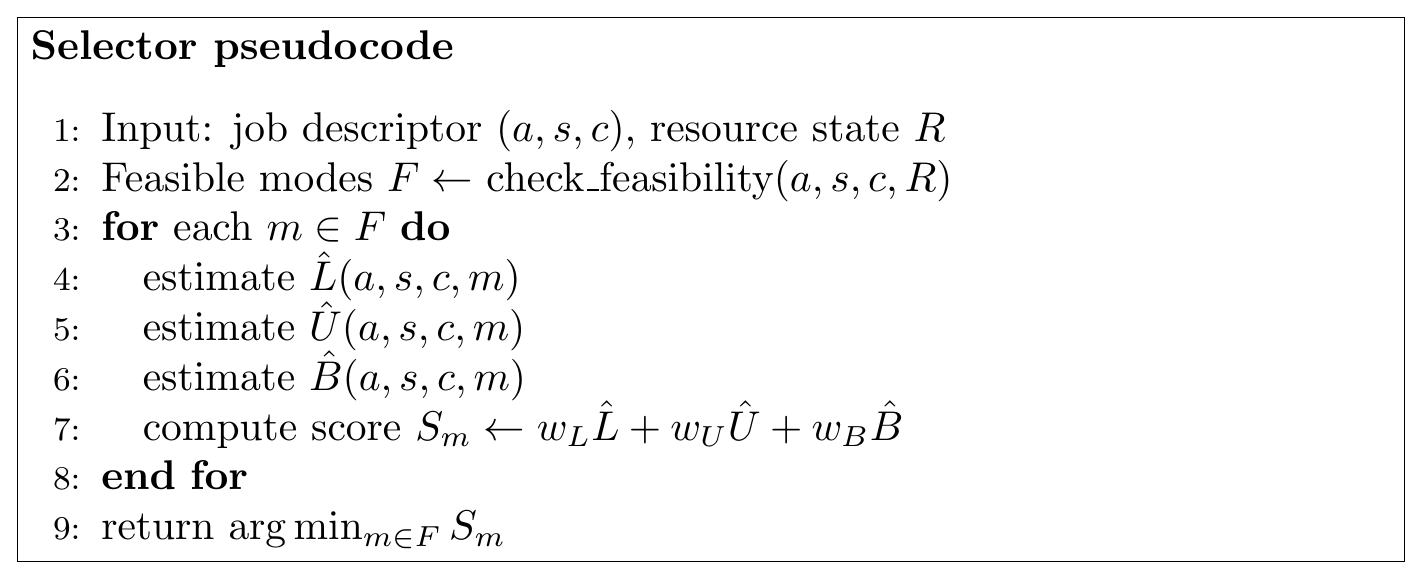
\includegraphics[width=\linewidth]{figures/pseudocode.png}
    \caption{Online weighted-cost selection logic.}
    \label{fig:pseudocode}
\end{figure}

In C++ terms, the selector used the following logic: for each candidate transfer mode, skip the mode if it is infeasible, evaluate the job with that mode, compute $C(j,m)$ using the active weights, and keep the minimum-cost mode. If no feasible mode is found, the implementation falls back to PIO for safety. This fallback is conservative because PIO is simple and does not require DMA state to be valid.

\subsection{Weight Configurations}
Three weight configurations were evaluated in simulation. The CPU-dominant configuration used $w_L=0.15$, $w_U=0.65$, and $w_B=0.10$, which prioritizes low CPU occupancy over raw latency. The latency-dominant configuration used $w_L=0.65$, $w_U=0.20$, and $w_B=0.15$, which prioritizes completion time while still considering CPU and bus effects. The equal-weight configuration treated latency, CPU occupancy, and bus pressure with approximately equal priority, using about one third of the total weight for each metric.

\section{Experimental Setup}
\subsection{Platform and Tools}
The original proposal targeted an STM32H745-class platform \cite{stm32h745}. The final hardware experiment was performed on an STM32F439ZI board with the on-chip CRYP AES hardware peripheral. Cycle measurements were taken with the MCU cycle counter and converted to microseconds using a 168 MHz system clock. UART logs were used to collect records such as payload size, cycle count, latency, throughput, checksum, selected mode, and regret.

The software implementation used C/C++ firmware-style code for the selector and AES measurement paths. The analysis and plot generation were performed offline from text/CSV logs. The project source code and related artifacts are available in a public \href{https://github.com/egekarakaya/CMP720-Data-Movement-Strategy-Selection-for-AES-ECDSA-Accelerator-Workloads-on-an-STM32H7-Series-MCU}{GitHub repository}.

\subsection{Workloads}
Two workloads were used:
\begin{itemize}
    \item \textbf{Simulation workload:} 1000 synthetic jobs over multiple payload sizes and contention classes. This workload evaluated PIO, DMA single-shot, DMA burst, and double-buffer choices under different weight configurations.
    \item \textbf{REAL\_3WAY AES measurement workload:} 50 measured AES jobs on the STM32F439ZI platform. The measured static paths were polling/PIO, DMA single-shot, and DMA burst with 256-byte chunks. Payload sizes included 16, 32, 64, 128, 256, 512, 1024, 2048, and 4096 bytes.
\end{itemize}

The real measurement workload did not include ECDSA and did not include true hardware double buffering. In the real 3-way experiment, the large-payload double-buffer region from the offline selector was mapped to the measured DMA burst path.

\subsection{Metrics and Baselines}
The main metrics were average latency, average throughput, aggregate throughput, CPU occupancy, bus pressure, regret relative to the best measured or oracle mode, and deadline-miss ratio. Throughput was computed as
\begin{equation}
\text{Throughput}_{\text{kB/s}} = \frac{\text{payload\_bytes}}{\text{time}_{\mu s}} \times \frac{1{,}000{,}000}{1024}.
\label{eq:throughput}
\end{equation}
Average throughput was computed by first calculating per-job throughput and then taking the arithmetic mean. Aggregate throughput was computed as total payload divided by total time.

The static baselines were always-PIO, always-DMA-single-shot, and always-DMA-burst. Adaptive selection was compared with the oracle in simulation and with measured static baselines in the real AES experiment.

\section{Results and Evaluation}
\subsection{Performance Results}
Table~\ref{tab:weight_results} summarizes the simulation results under three weight configurations. In all three configurations, the adaptive selector matched the oracle choices and achieved zero average regret. This shows that the cost-minimization logic correctly represented the offline oracle for the simulated model.

\begin{table}[ht!]
\centering
\caption{Simulation results for different adaptive weight configurations.}
\label{tab:weight_results}
\scriptsize
\begin{adjustbox}{width=\columnwidth}
\begin{tabular}{lrrrrr}
\toprule
\textbf{Configuration} & \textbf{Avg. latency ($\mu$s)} & \textbf{Avg. CPU ($\mu$s)} & \textbf{Avg. bus} & \textbf{Deadline miss} & \textbf{Regret} \\
\midrule
CPU-dominant & 303.117 & 16.616 & 10816 & 9.0\% & 0.000 \\
Latency-dominant & 299.711 & 17.203 & 10803 & 9.0\% & 0.000 \\
Equal weights & 299.755 & 17.163 & 10804 & 9.0\% & 0.000 \\
\bottomrule
\end{tabular}
\end{adjustbox}
\end{table}

The advantage of the adaptive selector over static strategies can also be observed from the simulated weighted cost. The cost-reduction ratio is computed as $(C_{\text{static}}-C_{\text{adaptive}})/C_{\text{static}}$. Table~\ref{tab:sim_cost_reduction} shows that the adaptive policy consistently reduced cost compared with fixed transfer strategies. The largest gain was obtained against static PIO, because PIO scales poorly for larger payloads. The adaptive selector also improved over static DMA single-shot and static DMA burst, although the margin became smaller when the best static baseline was static double buffer.

\begin{table}[ht!]
\centering
\caption{Simulated adaptive cost reduction relative to static baselines.}
\label{tab:sim_cost_reduction}
\scriptsize
\begin{adjustbox}{width=\columnwidth}
\begin{tabular}{lrrrr}
\toprule
\textbf{Configuration} & \textbf{vs. PIO} & \textbf{vs. DMA-SS} & \textbf{vs. DMA burst} & \textbf{vs. best static} \\
\midrule
CPU-dominant & 87.1\% & 26.3\% & 15.8\% & 5.1\% \\
Latency-dominant & 68.9\% & 32.3\% & 21.1\% & 1.1\% \\
Equal weights & 74.2\% & 29.6\% & 18.7\% & 1.8\% \\
\bottomrule
\end{tabular}
\end{adjustbox}
\end{table}

For the latency-dominant run, the adaptive average cost was 0.606. The corresponding static costs were 1.950 for static PIO, 0.894 for static DMA single-shot, 0.767 for static DMA burst, and 0.613 for static double buffer. Therefore, the adaptive policy was much better than the fixed PIO, DMA single-shot, and DMA burst policies, while still giving a small improvement over the best static baseline.

The weight configuration changed the selected modes even when the selector remained oracle-equivalent. With CPU-dominant weights, the selector chose double buffer for 438 jobs, DMA single-shot for 298 jobs, PIO for 211 jobs, and DMA burst for 53 jobs. With latency-dominant weights, double buffer increased to 590 selections, PIO increased to 252, DMA single-shot decreased to 158, and DMA burst was not selected. Equal weights behaved closer to the latency-dominant case, with 590 double-buffer selections, 166 DMA single-shot selections, 244 PIO selections, and zero DMA-burst selections. This behavior is shown in Fig.~\ref{fig:weight_distribution}.

\begin{figure}[ht!]
    \centering
    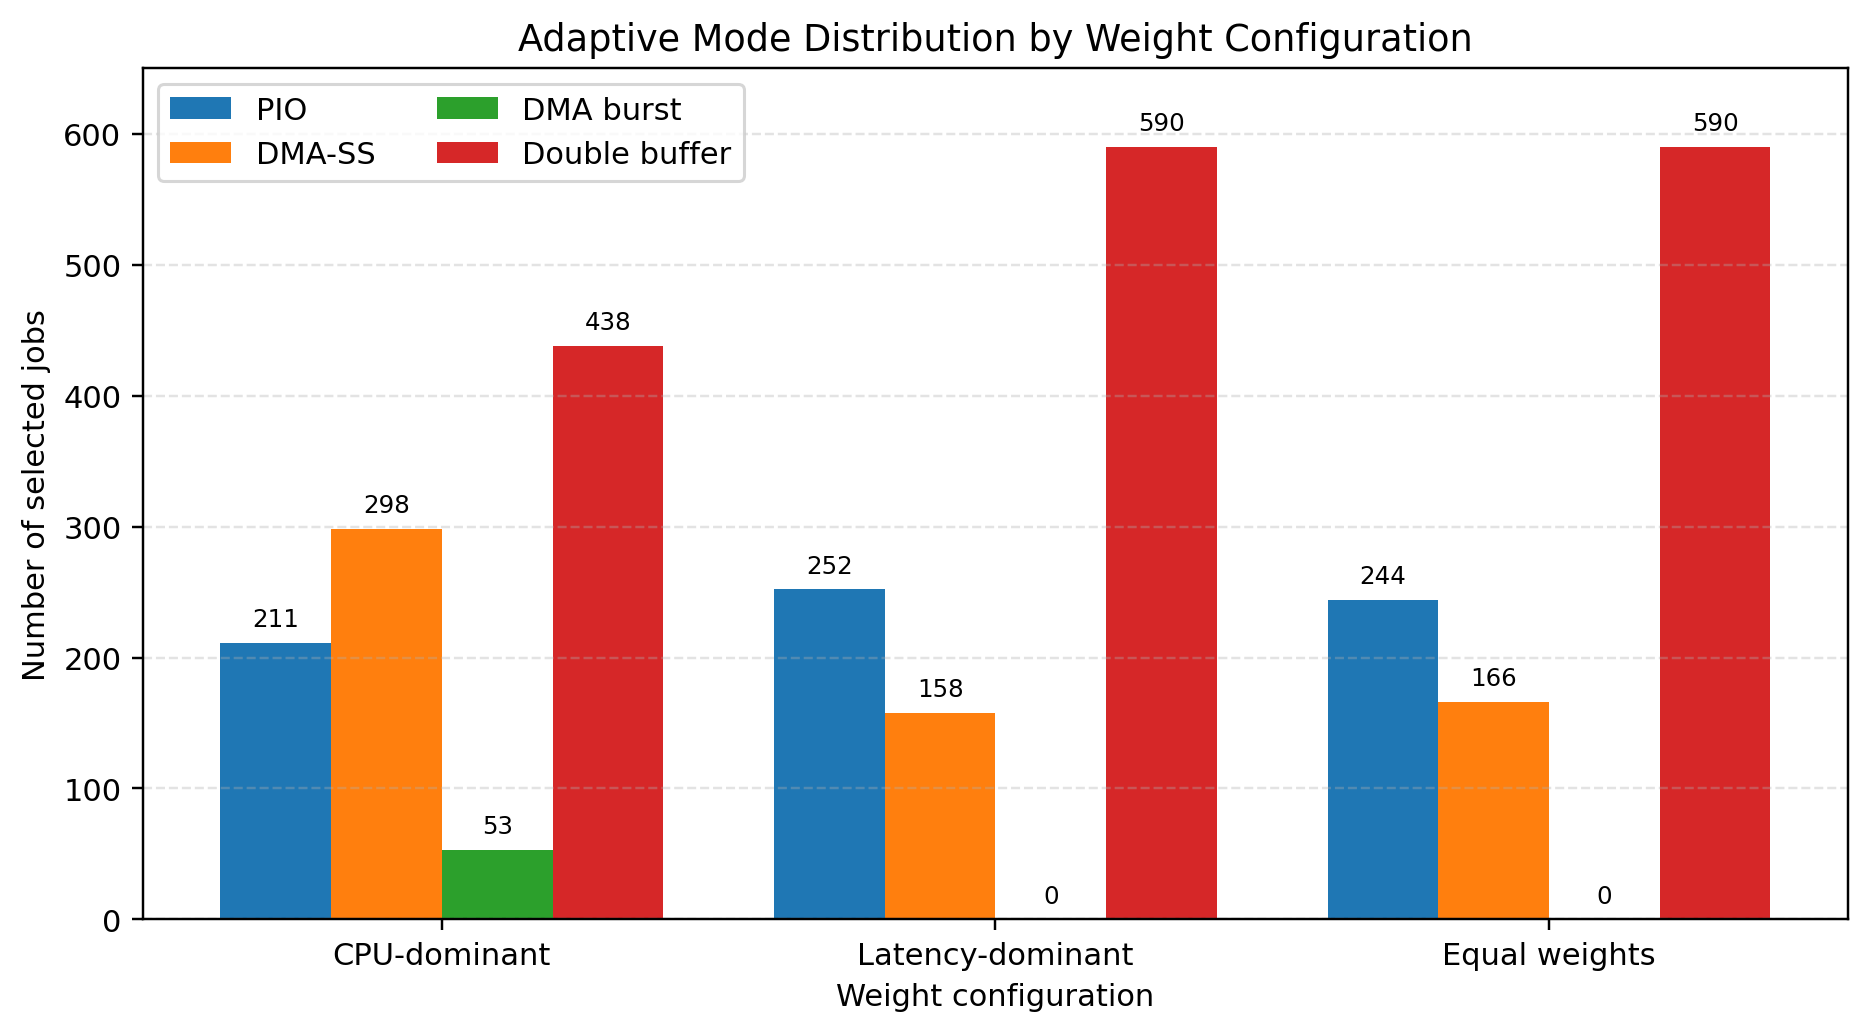
\includegraphics[width=\linewidth]{figures/weight_mode_distribution.png}
    \caption{Adaptive mode distribution under CPU-dominant, latency-dominant, and equal-weight configurations.}
    \label{fig:weight_distribution}
\end{figure}

Table~\ref{tab:real_static_adaptive} reports the real AES measurement comparison on 50 REAL\_3WAY jobs. Each static strategy was evaluated over the same job set. Adaptive selection used the selected mode for each job: PIO for tiny jobs, DMA single-shot for mid-sized jobs, and DMA burst for large jobs.

\begin{table}[ht!]
\centering
\caption{Static strategies versus adaptive selection on 50 REAL\_3WAY AES jobs.}
\label{tab:real_static_adaptive}
\scriptsize
\begin{adjustbox}{width=\columnwidth}
\begin{tabular}{lrrrr}
\toprule
\textbf{Strategy} & \textbf{Jobs} & \textbf{Avg. latency ($\mu$s)} & \textbf{Avg. throughput (kB/s)} & \textbf{Agg. throughput (kB/s)} \\
\midrule
Adaptive selection & 50 & 62.55 & 12{,}374.32 & 15{,}203.81 \\
Static PIO / polling & 50 & 279.82 & 3{,}035.92 & 3{,}398.42 \\
Static DMA single-shot & 50 & 23.37 & 26{,}785.27 & 40{,}691.22 \\
Static DMA burst & 50 & 63.18 & 11{,}045.40 & 15{,}051.81 \\
\bottomrule
\end{tabular}
\end{adjustbox}
\end{table}

Figure~\ref{fig:static_adaptive} visualizes the same comparison. Static PIO performed poorly because CPU-driven copying scaled badly as payload size increased. Static DMA burst had an average latency close to adaptive selection, but lower average throughput. Static DMA single-shot was best on the measured REAL\_3WAY workload, reaching 23.37~$\mu$s average latency and 26{,}785.27~kB/s average throughput. This is an important result because it shows that the real hardware measurements did not fully match the selector's offline assumptions for large jobs.

\begin{figure}[ht!]
    \centering
    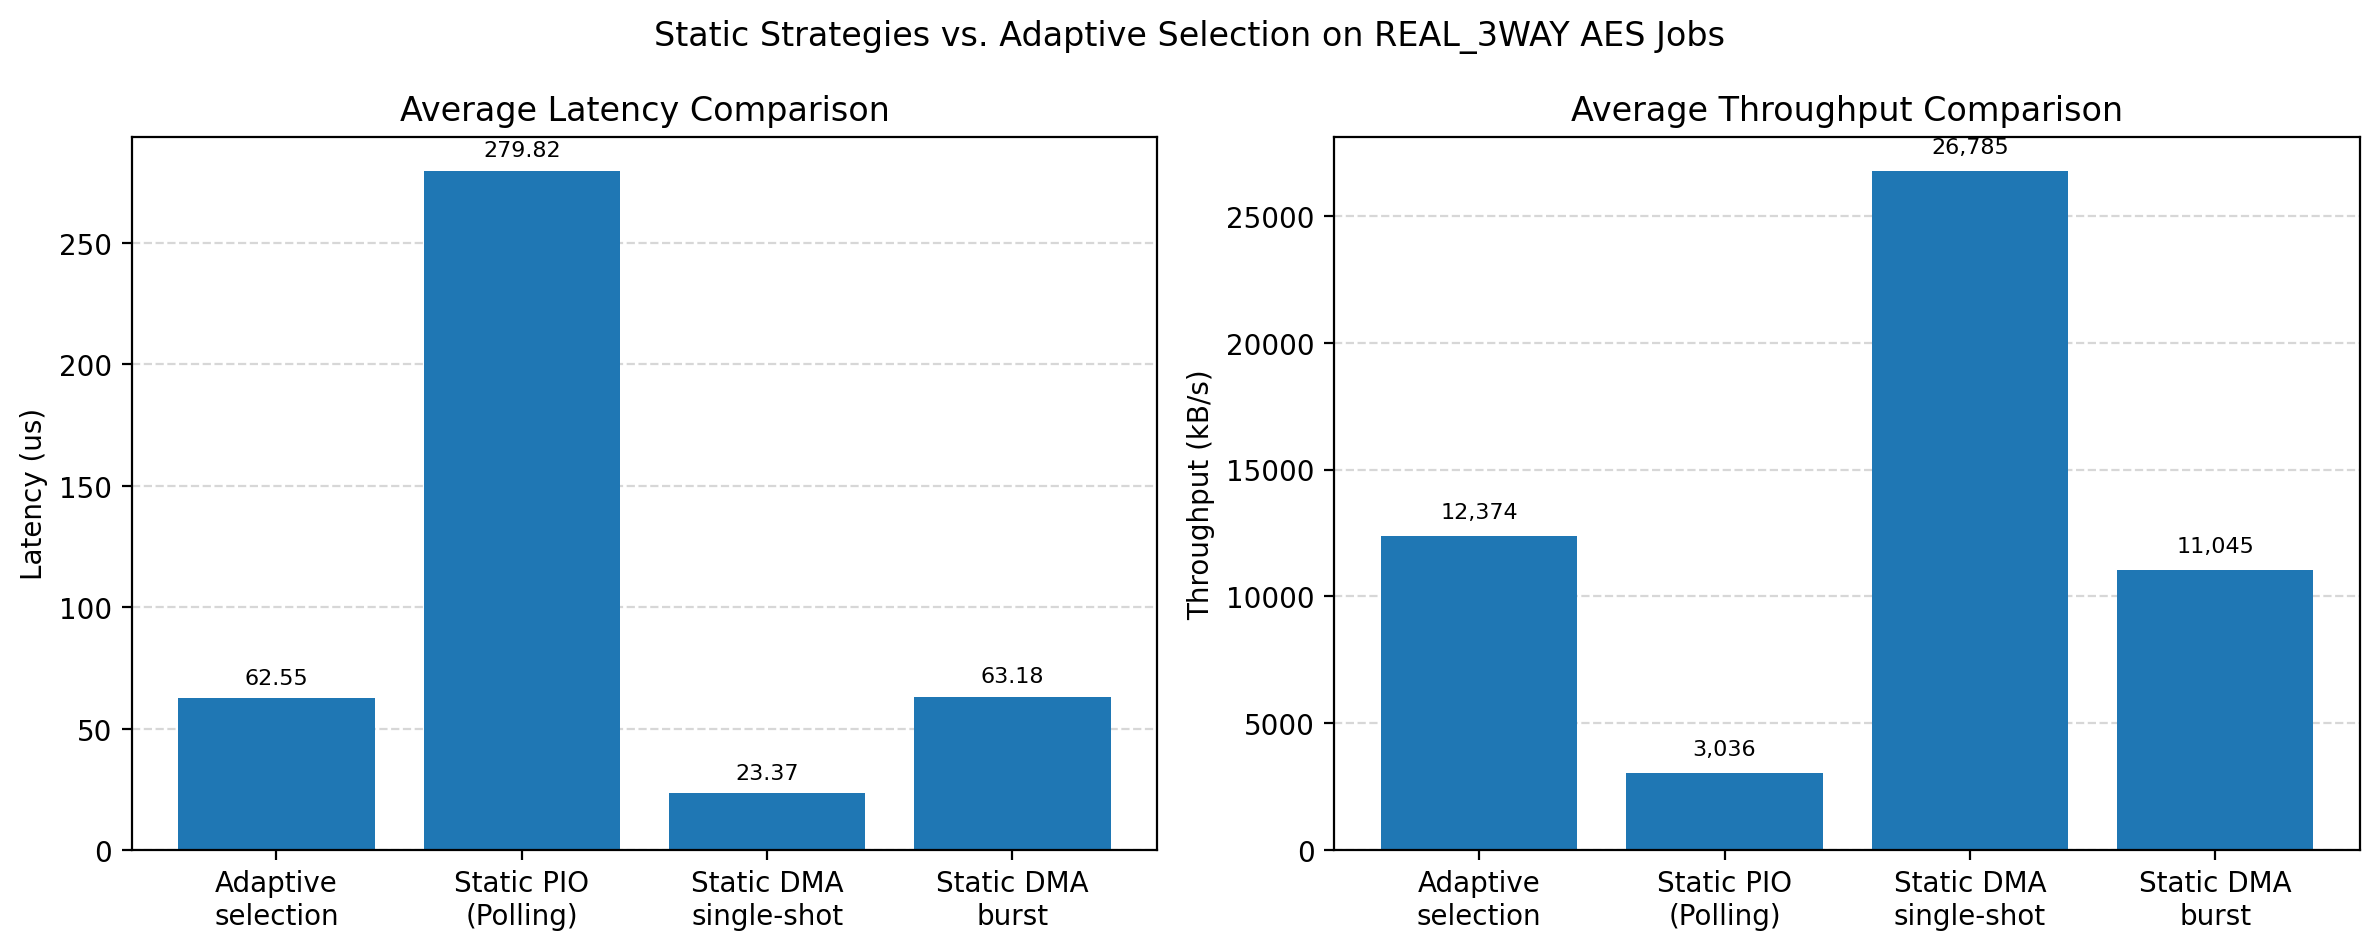
\includegraphics[width=\linewidth]{figures/static_adaptive_comparison.png}
    \caption{Average latency and throughput comparison between adaptive selection and static strategies on the measured AES workload.}
    \label{fig:static_adaptive}
\end{figure}

\subsection{Comparative Analysis}
The simulation and hardware results tell slightly different stories. In simulation, adaptive selection matched the oracle for all weight configurations. This indicates that the selector implementation correctly minimized the modeled weighted cost. The simulation also confirmed that weights matter: increasing the CPU weight delayed aggressive double-buffer selection, while latency-oriented and equal-weight configurations selected double buffering much earlier.

In the hardware measurement, adaptive selection clearly outperformed static PIO but did not outperform static DMA single-shot. Compared with adaptive selection, static PIO had approximately 347\% higher average latency and about 75.5\% lower average throughput. Static DMA burst had nearly the same average latency as adaptive selection, around 1\% higher, but about 10.7\% lower average throughput. Static DMA single-shot, however, was 62.6\% lower in latency and 116.5\% higher in average throughput than adaptive selection on this measured workload.

The main reason is that the final hardware experiment did not implement true double buffering. The offline large-payload region was mapped to DMA burst in the REAL\_3WAY run, while the measured best real mode for many large payloads was DMA single-shot. Therefore, the adaptive selector was correct with respect to its model, but the model was not perfectly calibrated to the measured STM32F439ZI behavior. This is not a failure of the optimization formulation; it is a calibration and implementation-gap result.

\subsection{Discussion}
Several parts of the project worked as expected. First, PIO was effective only for very small payloads, where DMA setup overhead can dominate. Second, DMA-based transfer became much better as payload size increased. Third, changing the cost weights changed the selector behavior in an interpretable way. CPU-dominant weights protected CPU occupancy, while latency-oriented weights selected more aggressive buffering strategies.

The main unexpected result was that static DMA single-shot was the strongest strategy in the real AES measurements. In the simulation model, larger payloads favored burst or double-buffer-style behavior. On the measured STM32F439ZI run, DMA single-shot had both the lowest average latency and the highest throughput over the 50-job workload. This suggests that burst management overhead and the absence of true overlap reduced the benefit of the burst path.

The most important limitation is the difference between the original architecture and the final hardware implementation. The proposal described an STM32H7-class platform with possible external or tightly coupled accelerator service and support for double buffering. The final measurement used STM32F439ZI AES CRYP hardware and did not implement true double buffering. Also, ECDSA was not measured. As a result, the final hardware evidence supports the data-movement methodology for AES, but not the full AES/ECDSA scope originally proposed.

From an embedded systems perspective, deadline miss is an important metric because it indicates whether a job is real-time feasible, not only whether it eventually completes. In the simulation runs, adaptive selection and oracle both had a 9.0\% deadline-miss rate. This suggests that missed deadlines came from jobs that exceeded the timing capacity of the modeled system, not from wrong mode selection. In the real 50-job AES run, using a 1100~$\mu$s reference deadline, the adaptive, static DMA single-shot, and static DMA burst paths did not miss the deadline, while static PIO would miss it for the 4096-byte cases. The exact deadline policy should be configured according to the final application.

\subsection{Reproducibility}
The experiments can be reproduced with the following information:
\begin{itemize}
    \item \textbf{Hardware:} STM32F439ZI board for the final AES CRYP measurement.
    \item \textbf{Clock assumption:} cycle counts were converted using a 168~MHz system clock.
    \item \textbf{Measured transfer modes:} polling/PIO, DMA single-shot, and DMA burst with 256-byte chunks.
    \item \textbf{Simulated transfer modes:} PIO, DMA single-shot, DMA burst, and double buffer.
    \item \textbf{Measured payload sizes:} 16, 32, 64, 128, 256, 512, 1024, 2048, and 4096 bytes.
    \item \textbf{Measured job set:} 50 REAL\_3WAY AES records including low, medium, and high contention labels.
    \item \textbf{Main formula:} throughput was computed with~\eqref{eq:throughput}.
    \item \textbf{CPU-dominant weights:} $w_L=0.15$, $w_U=0.65$, and $w_B=0.10$.
    \item \textbf{Latency-dominant weights:} $w_L=0.65$, $w_U=0.20$, and $w_B=0.15$.
    \item \textbf{Equal-weight configuration:} latency, CPU occupancy, and bus pressure were weighted approximately equally, using about $0.33$ for each metric.
    \item \textbf{Code availability:} The project source code and related artifacts are available in the public \href{https://github.com/egekarakaya/CMP720-Data-Movement-Strategy-Selection-for-AES-ECDSA-Accelerator-Workloads-on-an-STM32H7-Series-MCU}{GitHub repository}. The firmware source, UART logs, and analysis scripts should be archived with the submitted report package to reproduce the results exactly.
\end{itemize}
A classmate could reproduce the real measurement by running the AES benchmark firmware, collecting UART records for the same payload sequence, and recomputing latency and throughput per transfer strategy. The simulation results can be reproduced by generating the same synthetic job set, evaluating all feasible modes, applying the weighted-cost formula, and comparing the adaptive decision against the oracle minimum.

\section{Conclusion and Future Work}
This project investigated adaptive data movement for AES accelerator workloads on STM32-class embedded systems. The main idea was to treat transfer-mode selection as an optimization problem over latency, CPU occupancy, and bus pressure rather than as a fixed implementation choice. The project implemented a lightweight weighted-cost selector and evaluated it using both simulation and real AES measurements.

The strongest positive result is that the adaptive selector matched the oracle in simulation for CPU-dominant, latency-dominant, and equal-weight configurations. The simulations also showed that the chosen weights directly affect system behavior: CPU-dominant weights reduce CPU occupancy, while latency-oriented and equal-weight configurations select more double-buffer-style modes. This supports the claim that a tunable selector is useful in embedded systems where the optimization priority may change.

The real AES measurements produced a more cautious result. Adaptive selection avoided the poor scaling of static PIO and performed similarly to static DMA burst, but static DMA single-shot was the best measured baseline on the 50-job REAL\_3WAY workload. This means the final selector should not be overclaimed as universally better than all static baselines. Instead, the correct conclusion is that the selector framework works, but the cost model and thresholds must be calibrated with the actual hardware behavior. In particular, mapping the simulated double-buffer region to DMA burst was not sufficient to reproduce the expected benefit of true overlapped execution.

Several planned items were not completed. ECDSA was not measured, true hardware double buffering was not implemented, direct energy measurement was not performed, and queue-level scheduling was not studied. These are the main limitations of the current work.

Future work should implement true double buffering on the target platform, add ECDSA or another public-key workload, collect direct power measurements if possible, and retrain or retune the selector using real hardware profiles. A further extension would be to make the selector deadline-aware: first eliminate modes that cannot meet a job deadline, then minimize the weighted cost among feasible real-time choices. Finally, the project could be extended from per-job selection to queue-level scheduling when multiple cryptographic jobs compete for DMA, SRAM, and accelerator resources.

\section*{Acknowledgments}
The author would like to thank the course instructor for the feedback that helped refine the scope, structure, and system-level framing of this project.

\small
\begin{thebibliography}{99}

\bibitem{fips197}
NIST, ``Advanced Encryption Standard (AES),'' FIPS PUB 197, Nov. 2001, updated May 2023.

\bibitem{fips1865}
NIST, ``Digital Signature Standard (DSS),'' FIPS PUB 186-5, Feb. 2023.

\bibitem{silabs_dma}
Silicon Laboratories, ``AN0013: Direct Memory Access,'' Application Note, 2013.

\bibitem{arm_axi}
Arm, ``Introduction to AMBA AXI4,'' Issue 01, 2020.

\bibitem{zhang2021}
Z. Zhang \emph{et al.}, ``High-Efficiency Parallel Cryptographic Accelerator for Real-Time Data Security in Embedded Systems,'' \emph{Micromachines}, vol. 12, no. 5, p. 560, 2021.

\bibitem{agrawal2022}
R. Agrawal \emph{et al.}, ``Efficient FPGA-Based ECDSA Verification Engine for Permissioned Blockchains,'' in \emph{Proc. ACM/SIGDA Int. Symp. on Field-Programmable Gate Arrays}, 2022.

\bibitem{Saidi2012}
S. Saidi, P. Tendulkar, T. Lepley, and O. Maler, ``Optimizing explicit data transfers for data parallel applications on the cell architecture,'' \emph{ACM Transactions on Architecture and Code Optimization}, vol. 8, no. 4, pp. 1--20, Jan. 2012.

\bibitem{Mera2022}
A. Mera, Y.-H. Chen, R. Sun, E. Kirda, and L. Lu, ``D-Box: DMA-enabled compartmentalization for embedded applications,'' \emph{arXiv preprint arXiv:2201.05199}, 2022.

\bibitem{Rodrguez2018}
A. Rodriguez \emph{et al.}, ``FPGA-Based High-Performance Embedded Systems for Adaptive Edge Computing in Cyber-Physical Systems: The ARTICo$^3$ Framework,'' \emph{Sensors}, vol. 18, no. 6, p. 1877, 2018.

\bibitem{Zulberti2024}
G. Corradi, M. Cattaneo, and S. Di Carlo, ``SmartDMA: Adaptable Memory Access Controller for Specialized Architectures in Edge Computing,'' preprint, 2024.

\bibitem{Montanaro2022}
G. Montanaro, A. Galimberti, E. Colizzi, and D. Zoni, ``Hardware-Software Co-Design of BIKE with HLS-Generated Accelerators,'' arXiv:2209.03830, 2022.

\bibitem{stm32h745}
STMicroelectronics, ``STM32H745xI/G Dual-Core Arm Cortex-M7 and Cortex-M4 MCUs Datasheet,'' Rev. 3, Jan. 2026.

\end{thebibliography}
\normalsize

\end{document}
